%% ------------------------------------------------------------------------- %%
\chapter{Conceitos}
\label{cap:conceitos}



Explicar gigapixel
explicar gpgpu
explicar registro
explicar os algoritmos estudados

%% ------------------------------------------------------------------------- %%
\section{Registro}\index{Registro}
\label{sec:fundamentos}

    O registro de imagens tem como objetivo encontrar um alinhamento entre duas imagens diferentes. Dada duas imagens, 
a imagem Referência (R) e a imagem Alvo (A), os algoritmos de registro encontram um campo
vetorial de deslocamento que é aplicado a imagem Alvo, movendo seus pixels para um estado no qual ela esteja alinhada
com a imagem Referência.



Podemos definir o processo de registro com a seguinte equação, como \cite{brown1992survey} fez em seu estudo:
\begin{align}\label{eq:defregistro}
    R(x,y) = g(A(f(x,y)))
\end{align}
    Representamos uma imagem como uma matriz de pixels e acessamos seus pixels utilizando a seguinte convenção $R(x,y)$ 
que nos dá o pixel da imagem $R$ na possição $(x,y)$. $f(x,y) = (x',y')$ é uma função que representa o deslocamento do 
campo vetorial encontrado pelo registro e $g$ é uma função que modifica a intensidade dos pixels, se for necessário. 
Cada algoritmo de registro utiliza um método diferente para encontrar a função de transformação $f$, mas os passos gerais são:
\begin{enumerate}
    \item Pré-processamento;
    \item Detecção de caracteristicas;
    \item Correspondência de caracteristicas;
    \item Estimação da função de transofrmação;
    \item Reamostragem da imagem Alvo.
\end{enumerate}
    É importante salientar que nem todos algoritmos de registro seguem essa lista a risca, e mesmo que sigam eles ainda
podem realizar mais de um passo por vez. Os passos gerais são representados na imagem \ref{fig:regExplicacao}. 
Vamos tratar brevemente dos passos nas seções abaixo.
\begin{figure}[H]
    \centering
    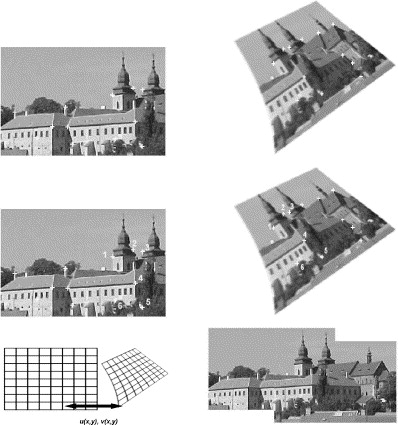
\includegraphics[width=0.8\textwidth]{figuras/regSteps.jpg}
    \caption{Na primeira linha estam a imagem referência e a alvo, respectivamente. Na segunda linha as características
da imagem referência foram encontradas e suas correspondentes na imagem Alvo. A última linha mostra a estimação da 
função e a sua reamostragem da imagem Alvo. \citep{zitova2003image}}
    \label{fig:regExplicacao}
\end{figure}

%% ------------------------------------------------------------------------- %%
\subsection{Pré-processamento}
    Essa é a etapa mais aberta dentre todas. Antes de iniciar o processo de registro, é possível que as imagens tenham
que passar por algum processamento para melhorar o resultado final do registro. Esse pré-processamento muda de acordo
com as necessídades de cada caso. Se temos imagens com muito ruido, essa é a hora de aplicar filtros para melhorar sua 
qualidade. Certos algoritmos de registro não trabalham com as imagens, e sim com segmentações delas ou somente com suas
bordas, então a aquisição desses dados é feita nessa etapa.

%% ------------------------------------------------------------------------- %%
\subsection{Detecção de caracteristicas}\index{Detecção de caracteristicas}
\label{sec:dec_corr_carac}

    Com as imagens já pré-processadas, o primeiro passo para um algoritmo de registro é a localização de estruturas de 
destaque dentro de uma cena ou de um objeto. Tais estruturas devem ser facilmente identificadas em fotos obtidas sob 
outra perspectiva ou ângulação. Elas são separadas em 3 grupos:

\textbf{Características de Região} - São demarcadas como regiões de alto contraste dentro da imagem. Lagos, florestas ou
regiões urbanas são exemplos desse tipo de característica. Sua detecção é feita utilizando algoritmos de segmentação.

\textbf{Características de Linha} - São linhas encontradas dentro da imagem. Podem ser ruas, rios ou o litoral. Métodos
clássicos de detecção de bordas como o Canny ou o filtro laplaciano são usados para identificar essas características.

\textbf{Características de Ponto} - São pontos de intersecção entre linhas, representados por intersecções de ruas ou
rios, ou pontos de máxima curvatura. Algoritmos para identificação de pontos utilizam técnicas mais avançadas, dada a 
dificuldade de encontrá-los. Os mais básicos encontram as intersecções de linhas enquanto os mais avançados buscam
centróides de regiões ou o máximo local de uma \textit{wavelet}.

    Dada a importância desse passo, vários algoritmos foram desenvolvidos com o passar dos anos para resolver de maneira
rápida e eficiente a detecção de caracteristicas. Alguns dos mais famosos, como o 
\textit{Scale Invariant Feature Transform} (SIFT) , introduzido por \cite{lowe1999object}, transforma uma imagem em uma 
coleção de vetores de caracteristicas locais, que são usados para identidicar as caracteristicas. Outro algoritmo famoso,
desenvolvido por \cite{bay2006surf}, o \textit{Speeded Up Robust Features} (SURF) utiliza o determinante da matriz de
Hessian para identificar regiões da imagem que tenham um valor diferenciado para alguma propriedade, como brilho, de 
regiões vizinhas. Ao identificar uma região, ele cálcula a caracteristica dela utilizando a soma dos 
\textit{Wavelets de Haar}.

%% ------------------------------------------------------------------------- %%
\subsection{Correspondência de caracteristicas}\index{Correspondência de caracteristicas}

    Com as caracteristiscas de cada uma das imagens encontradas, o próximo passo é realizar a correspondencia entre elas.
A primeira soluço a ser apresentada, a Correspondência por Área, mescla o passo de Detecção com o de Correspondência. 
Ele utiliza duas janelas, uma para cada imagem, de formato retangular ou circular, e utiliza metricas para enumerar a 
relação entre elas. O algoritmo então move as janelas dentro das imagens afim de encontrar o par que tem a máxima
relação entre si. Várias métricas podem ser utilizadas, como a Correlação entre as intensidades das janelas, o estudo
do spectro da transformada de \textit{Fourier} das janelas ou o cálculo da informação mutua entre elas. 

 Outro grupo de algoritmos recebe como entrada dois conjuntos de caracteristicas e estabelece as correspondências
usando relações espaciais entre as caracteristicas de conjuntos diferentes. Cada algoritmo dentro desse grupo 


    
\section{Computação de Alto Desempenho}
    Para criar a imagem \textit{Gigapixel} um algoritmo de registro é executado $(n_c-1)*(n_l-1)$ vezes no minimo, 
onde $n_c$ e $n_l$ são o número de colunas e linhas de fotografias que compõem a imagem \textit{Gigapixel}, 
respectivamente. Esse número é uma estimativa otimista, já que mais processos de registro são potencialmente executados
entre fragmentos para melhorar a qualidade da imagem final. Uma das maiores imagens \textit{Gigapixel} até hoje, 
o projeto \textit{Servilla 111 Gigapixels}, coordenado por \cite{sevilla111},  conta com 9,750 fotografias, dispostas
em 65 linhas. Nesse projeto foram executados, no melhor dos casos, 9536 registros entre fotos de 22 \textit{Megapixels}
, algo claramente custoso.

    Podemos acelerar o processo de custura das imagens usando várias abordagens diferentes. A mais clássica seria
paralelizar o algoritmo inteiro, utilizando a grande capacidade das \textit{CPUs} atuais em executar processos paralelos.
Outra abordagem é atacar diretamente o passo do registro, construindo algoritmos menos custosos ou melhorar algoritmos
existentes. A abordagem escolhida foi modificar o TPS, criando uma versão que segue a arquitetura 
\textit{Single Instruction Multiple Data} (SIMD). A escolha foi feita pensando em uma implementação para 
Unidades de Processamento Gráfico (\textit{Graphic Processing Units} (GPUs)).

\subsection{Unidade de Processamento Gráfico}
    A GP nasceu da necessidade dos antigos \"arcades\" de renderizar cenas complexas mantendo uma taxa de quadros por 
segundo aceitavel para o jogador. Elas são placas lógicas criadas ao redor de um Na decada de 90 as GPUs foram levadas para o computador pessoal, incrementando 

A placa contém um escalonador para threads implementado em hardware. Ele é responsável por escalonar as threads que serão
executadas nos streaming multiprocessors (SM). Um SM é um conjunto de 48 processadores, um pequeno bloco de memória própria,
um cache de instruções e 8 unidades de funções gráficas. A Geforce GTX 460 tem 7 SMs, totalizando 336 processadores.

O código que será executado em cada processador é chamado de \textbf{kernel}. Ao executar um kernel na GPU, o 
hardware criará threads, cada uma delas executando o mesmo código, mas com dados diferentes. Nas placas NVIDIA as threads 
são agrupadas em blocos, e esses blocos são escalonados para cada SM. Depois, todas as threads dentro de um bloco são 
divididas em pequenos grupos chamados de \textbf{warp}\cite{paulo}, e cada warp é executado paralelamente dentro do 
mesmo SM para qual o bloco foi escalonado. Existe um limite para a quantidade de threads escalonadas para execução
dentro de um SM, que é definida pelos recursos que cada thread consome. Por exemplo, não há como executar 10 threads
que consomem 10 registradores cada em um SM com 90 registradores.

Outra parte importante do hardware é a memória, que é limitada em relação à da CPU. GPUs tem, em média, 1GB
de memória, enquanto CPUs tem 4GB. O acesso a um mesmo bloco de memória é concorrente, mas ao utilizar caches e leitura ou escritas em
conjunto podemos minimizar a taxa com que leituras ou escritas conflitantes são feitas. Mas ainda sim é necessário atenção ao escrever um
kernel. Dada a estrutura do hardware da GPU, é melhor deixar threads que façam operações sobre posições de memória próximas no mesmo
SM, assim elas podem utilizar a memória compartilhada do mesmo, e elas podem requisitar em conjunto um mesmo bloco da memória principal,
se necessário.

No caso da GTX460 cada SM tem um bloco de memória de 64KB. Esse bloco pode ser configurado para 16KB de memória compartilhada e 48KB
de cache L1 ou vice versa. A memória principal da placa é de 1024MB com conexões de 256 bits. A placa também tem um
cache L2 de 512KB.

Outro fator limitante é a transferência de dados da memória principal do computador para a memória 
principal da GPU. A transmissão é feita por um barramento PCI Express, com velocidades de até 16GB/s ( dado que o
barramento seja utilizado somente pela GPU ). Essa transmissão é a parte mais lenta de todo o
processo de execução na GPU e dado isso, em alguns casos é mais viável executar na GPU um pedaço do seu programa que seria executado
na CPU do que retornar os dados computados na GPU para a CPU, executar esse pedaço especifico, e passá-los de volta para a GPU 
para mais operações e novamente retornar esses dados para a CPU no final, passando duas vezes a mais pelo PCI Express. 

Ao estudar como o código é executado nas GPUs NVIDIA descobrimos a existência de uma máquina virtual chamada de Parallel Thread Execution\cite{ptx}.
Todo kernel é primeiro compilado para um arquivo .ptx que é executado na GPU através da máquina PTX. Ela é utilizada para garantir 
a retrocompatibilidade de kernels em placas mais antigas.
\subsection{Single Instruction Multiple Data}

\subsection{CUDA}
\textit{Compute Unified Device Architecture}, definida pela (CUDA) é uma arquitetura de programação para GPUs criada 
pela ~\cite{nvidia2007compute}.
Ele adiciona suas diretrizes para as linguagens C, C++, FORTRAN e Java, permitindo que elas usem a GPU.
Esse trabalho usa o CUDA junto com a linguagem C.
A versão 1.0 do CUDA foi disponibilizada no inicio de 2007. Atualmente só existe um compilador para CUDA, o nvcc,
e ele só da suporte para GPUs NVIDIA.

Para uma função executar na GPU ela precisa ser invocada de um programa da CPU. Chamamos esse programa de \textit{Host}
e a GPU onde o kernel irá executar de \textit{Device}.

O CUDA implementa um conjunto virtual de instruções e memória, tornando os programas retroativos. O compilador
primeiro compila o código em C para um intermediário, chamado de PTX, que depois será convertido em linguagem
de máquina. Na conversão do PTX para linguagem de máquina o compilador verifica quais instruções o \textit{device}
suporta e converte o código para usar as instruções corretas.
Para obter o maior desempenho possível, é importante saber para qual versão o código final será compilado, 
pois na passagem do código de uma versão maior para uma menor não existe a garantia que o algoritmo seguira as mesmas instruções, 
o compilador pode mudar um conjunto de instruções para outro menos eficiênte, ou em alguns casos, algumas instruções não existem em
versões mais antigas do hardware.

\subsubsection{Modelo de Plataforma}
A inicialização dos recursos que o CUDA necessita para a comunicação com a GPU é feita no background da
aplicação no momento da primeira chamada de alguma das diretivas do CUDA. Essa primeira diretiva terá um
tempo maior de execução que chamadas subsequentes a mesma diretiva. Na inicialização o CUDA identifica
os \textit{devices} existentes e escolhe um deles para ser o responsável pelas execuções posteriores.

O próximo passo é a alocação de memória no \textit{device}. As operações de leitura de memória de um kernel são feitas somente
na memória de um \textit{device}. A alocação dessa memória é feita pelo \textit{host}, usando \verb#cudaMalloc()#. 
Para copiar a memória do \textit{host} para o \textit{device} ou vice-versa,
\verb#cudaMemcpy()# é usada. Para liberar o espaço alocado após a execução basta usar o \verb#cudaFree()#.
Todas essas diretivas recebem um ponteiro do \textit{host}, usado para o controle sobre qual posição da memória está sendo
operado em cada operação.

O CUDA dá suporte a alocação de vetores em duas ou três dimensões através de: \verb#cudaMallocPitch()# e 
\verb#cudaMalloc3D()#, respectivamente. É necessário usar as modificações dos comandos \verb#Memcpy# para
duas ou três dimensões também, que são: \verb#cudaMemcpy2D()#, \verb#cudaMemcpy3D()#.

\subsubsection{Modelo de Programação}
Um kernel no CUDA é uma função C que será executada paralelamente $n$ vezes em $n$ threads diferentes na GPU. Um kernel pode ser
definido em qualquer lugar do seu código, usando a declaração \verb#__global__# do lado esquerdo do tipo de retorno do kernel.
Para invocar um kernel, o \textit{host} faz a chamada de uma função com a sintaxe parecida com o C, mas usa uma configuração de
execução definida pelo CUDA, que usa a sintaxe \verb#<<<...>>># junto da chamada da função. Os parâmetros da configuração são
o número de blocos de threads e o número de threads por blocos. Para somar dois vetores de tamanho M e guardar o resultado num
outro vetor, o código é o seguinte:

\begin{lstlisting}
  __global__ void MatrixMulti ( float* a, float* b, float* c) { 
    int i = threadIdx.x;
    a[i] = b[i] + c[i];        
  }
                            
  int main () {               
    ...                       
    VecAdd<<<1,M>>>(a, b, c)  
    ...                       
  }                                 
\end{lstlisting}

No kernel acima, a linha \verb#int i = threadIdx.x# atribui a variável i o valor do indice da thread atual na primeira dimensão. 
A estrutura \verb#threadIdx# é um vetor de 3 dimensões, logo as threads podem ser organizadas em 1, 2 ou 3 dimensões dentro de um
\textit{device}. As threads são organizadas por blocos. Cada bloco tem dimensões maleáveis, mas as GPUs atuais limitam para 1024 o 
número máximo de threads por blocos. Cada bloco é lançado para execução em um processador diferente. Blocos são organizados em 
grids, que tem seu tamanho configurado na chamada o kernel, bem como o tamanho de cada bloco. No nosso exemplo acima, na linha
\verb#VecAdd<<<1,M>>>(a,b,c)#, o 1 determina o número de blocos e o M o número de threads por bloco.

O CUDA supõem que todos os blocos podem ser executados de maneira independende, ou seja, eles podem executar tanto paralelamente
quanto sequencialmente. Com isso, é possivel que o desempenho do código aumente em GPUs com mais processadores, sem que o programador
tenha que modificar o código.

O CUDA sabe qual instruções ele pode executar dentro de um \textit{device} baseando-se no seu Compute Capability 
(Capacidade Computacional). A Compute Capability de um \textit{device} são dois números, um que representa a arquitetura do 
\textit{device}, e outro que representa melhorias numa arquitetura.
A arquitetura \textit{Tesla}, a primeira da NVIDIA a dar suporte a GPGPU, tem Compute Capability 1.x, a seguinte, a \textit{Tesla},
tem 2.x e a atual, a \textit{Kepler}, tem 3.x. Dentro de cada arquitetura, podem existir melhorias nas instruções, que são
refletidas no número após o ponto, ou seja, uma placa com Compute Capability 2.1 tem instruções que uma 2.0 não tem.

\subsubsection{Hierarquia de Memória}
No CUDA, a memoria é separada lógicamente em 4 locais:

\begin{itemize}
  \item Registradores - Toda variável de uma thread fica em registradores.
  \item Memória Local - Memória acessivel por cada thread separadamente, mas de uso pouco provável. Ela só é usada se
          não existe mais espaço nos registradores ou se o compilador não ter certeza sobre o tamanho de um vetor.
  \item Memória Compartilhada - Cada bloco de threads tem uma memória compratilhada. A memória compartilhada é separada em
          pequenos blocos independentes. Se uma requisição de leitura tem n endereços em n blocos diferentes, o tempo de leitura
          desses n endereços é igual ao tempo de leitura de 1 endereço. Caso duas leituras caiam no mesmo bloco, elas serão
          serializadas. A memória compatilhada fica em chips dentro dos SMs, logo seu acesso é mais rápido do que o acesso a
          memória global.
  \item Memória Global - A memória global é acessivel por qualquer bloco em execução em um \textit{device}. A memoria global não é
          resetada após a execução de um kernel, então chamadas subsequentes de um mesmo kernel simplesmente leêm os resultados
          da memória global. Existe um pedaço da memória global reservada para valores constantes do programa.
\end{itemize}

Por padrão, o compilador do CUDA cuida do gerenciamento da memória, ou seja, ele é o responsável por distribuir os dados 
entre os locais diferentes de memória. O programador pode dar dicas para o compilador usando qualificadores indicando o local
que ele quer que aquele elemento fique na memória. Os possiveis qualificadores são:
\begin{itemize}
  \item \verb#__device__# Fica na memória global.
  \item \verb#__constant__#   Fica na area constante da memória global.
  \item \verb#__shared__# Fica na memória compartilhada das threads.
  \item \verb#__restrict__# Indica para o compilador que todos os ponteiros com esse qualificador apontam para locais diferentes
                            da memória. Isso é importante pois o compilador pode fazer otimizações com o código sabendo dessa informação.   
\end{itemize}

GPUs com Compute Cabapility maior ou igual a 2.0 podem alocar memória dentro do \textit{device} em tempo de execução.